\documentclass{article}
\usepackage{neurips_2024}
\usepackage{graphicx}
\usepackage{amsmath}
\usepackage{amsfonts}
\usepackage{hyperref}
\usepackage{url}
\usepackage{booktabs} % For formal tables
\usepackage{float} % For table and figure placement
\usepackage{cite}
\usepackage{natbib}


% Add the bibliography style to support author-year citations
\bibliographystyle{plainnat}


\title{Learning Disentangled Representations for Audio Classification}
\author{
  Nehemiah Skandera \\
  UC San Diego \\
  nskandera@ucsd.edu
}

\begin{document}

\maketitle

\begin{abstract}
Much of this CSE 192 course has been centered around how we can manipulate and visualize the unique features of audio to develop our understanding of how audio signals behave. Thus, we see that digital audio manipulation can be a challenging task - especially as it relates to Machine Learning. Furthermore, we can generalize that the task of classifying audio is especially challenging. According to the information I have found in my limited research, typical audio classification methods struggle with details such as feature extraction, and the disentangling of more pronounced audio frequencies. This project has been a journey of taking steps to explore the combination of Convolutional Neural Networks (CNN) with Support Vector Machines (SVM), and taking ideas from other papers to improve the model - such as generating disentangled representations of data. The objective of this project is to develop a model that learns disentangled versions of content, rhythm, and pitch from audio signals in order to integrate the corresponding representation into a hybrid CNN-SVM framework that attempts to enhance/discover the performance of classification mechanisms.
\end{abstract}

\section{Introduction}
The classification of audio signals is fundamental to many real-world applications. For instance, we use audio classification in speech recognition, oceanic research, and music recognition. However, we often see the limits of these systems of classification; often, complexity is overlooked. What makes this project (which was mostly a process of discovery) unique is that it introduces a novel approach that combines CNNs and SVMs and leverages disentangled signal representations in attempting to improve the performance of audio classification.


\section{Related Works}
\subsection{Learning Disentangled Representations for Timber and Pitch in Music Audio}
\citet{disentangled_representations} Disentangling timber and pitch in audio signals forms the basis for understanding the importance of disentangled features in audio classification.

\subsection{Unsupervised Speech Decomposition via Triple Information Bottleneck}
\citet{speech_decomposition} This paper investigates the use of information bottlenecks (hence the name) for unsupervised speech decomposition. Thus, providing information on how we can disentangle audio representations and enhance the extraction of audio features.


\section{Data Description}
\label{sec:data_description}
The dataset used in this project is gathered from room impulse responses (RIRs) in addition to noise sources from various databases. All of the data was gathered with a 16k sampling rate and 16-bit precision. Here is a description of the folders and data sources based on the data's README:

\subsection{Real RIRs and Isotropic Noises}
This set of real RIRs includes three databases:
\begin{itemize}
  \item \textbf{RWCP Sound Scene Database}
  \item \textbf{2014 REVERB Challenge Database}
  \item \textbf{Aachen Impulse Response Database (AIR)}
\end{itemize}
Overall, there are 325 real RIRs. The isotropic noises available in these databases are used in conjunction with their associated RIRs. The data can be downloaded from the following links:
\begin{itemize}
\item AIR: \url{http://www.openslr.org/resources/20/air_database_release_1_4.zip}
    \item RWCP: \url{http://www.openslr.org/resources/13/RWCP.tar.gz}
    \item 2014 REVERB Challenge: \url{http://reverb2014.dereverberation.com/tools/reverb_tools_for_Generate_mcTrainData.tgz} \\
    \url{http://reverb2014.dereverberation.com/tools/reverb_tools_for_Generate_SimData.tgz}
\end{itemize}

\subsection{Simulated RIRs}
This folder contains simulated RIRs. Details regarding this dataset can be found in the following `$simulated_rirs/README$` file. The simulated RIR dataset can be downloaded here:
\begin{itemize}
\item \url{http://www.openslr.org/resources/26/sim_rir.zip}
\end{itemize}

\section{Architecture}
\subsection{System Overview}
The proposed system for my project integrates feature extraction using Fourier Transforms and creates a disentangled representation for learning through CNNs. Classification is then accomplished using a hybrid CNN-SVM model.

\subsection{Components}
\begin{itemize}
  \item \textbf{Feature Extraction}: Fourier Transforms are used to extract frequency-domain features from audio signals.
  \item \textbf{Disentangled Representations}: The CNN-based encoder functions by extracting the content, rhythm, and pitch from audio signals.
  \item \textbf{Hybrid Model}: The CNN decoder functions by integrating the disentangled features. Meanwhile, the SVM classifier is used for further classification of the Fourier-transformed features.
\end{itemize}

\subsection{Implementation Details}
The system uses Python libraries such as `joblib` for faster computing times, TensorFlow, scikit-learn, and scipy for audio processing. Key components of the system include data preprocessing, feature extraction, model training, and model analysis.

\section{Experiments}
\subsection{Experimental Setup}
The dataset used for the experiments is described in Section~\ref{sec:data_description}. The dataset uses both real and simulated RIRs, in addition to isotropic noises. The dataset was divided into training and testing subsets, and the system's performance was evaluated based on classification accuracy.

\subsection{Methodology}
The methodology can be broken into steps:
\begin{itemize}
\item \textbf{Step 1}: Download and extract the dataset
\item \textbf{Step 2}: Load dataset RIR data
\item \textbf{Step 3}: Extract Fourier transforms as features
\item \textbf{Step 4}: Apply PCA for dimensionality reduction
\item \textbf{Step 5}: Data Augmentation
\item \textbf{Step 6}: Create Encoders
\item \textbf{Step 7}: Create CNN Decoder
\item \textbf{Step 8}: SVM Kernel System
\item \textbf{Step 9}: Bringing everything together
\item \textbf{Step 10}: System Evaluation
\end{itemize}

\subsection{Evaluation Metrics}
Accuracy is used as a metric to evaluate the performance of the CNN, SVM, and combined models.

\section{Results}
\subsection{Results Presentation}
\begin{itemize}
  \item \textbf{SVM Accuracy}: The SVM classifier achieved an accuracy of 92\% on the test set.
  \item \textbf{CNN Accuracy}: The CNN model achieved an accuracy of 61\% on the test set.
  \item \textbf{Combined Model Accuracy}: The combined model achieved an accuracy of 85\%.
\end{itemize}

\subsection{Confusion Matrix}
\begin{table}[H] % Use H to force placement
\centering
\begin{tabular}{lccc}
\toprule
\textbf{True \textbackslash Predicted} & \textbf{RVB2014} & \textbf{RWCP} & \textbf{air} \\
\midrule
\textbf{RVB2014} & 22 & 5  & 0 \\
\textbf{RWCP} & 0  & 40 & 0 \\
\textbf{air} & 0  & 8  & 9 \\
\bottomrule
\end{tabular}
\caption{Confusion matrix showing the number of true vs. predicted classifications for each class.}
\label{tab:confusion_matrix}
\end{table}

\subsection{Classification Report}
\begin{table}[H] % Use H to force placement
\centering
\begin{tabular}{lcccc}
\toprule
\textbf{Class} & \textbf{Precision} & \textbf{Recall} & \textbf{F1-score} & \textbf{Support} \\
\midrule
RVB2014 & 1.00 & 0.81 & 0.90 & 27 \\
RWCP & 0.75 & 1.00 & 0.86 & 40 \\
air & 1.00 & 0.53 & 0.69 & 17 \\
\midrule
\textbf{Accuracy} & \multicolumn{4}{c}{0.85} \\
\textbf{Macro avg} & 0.92 & 0.78 & 0.82 & 84 \\
\textbf{Weighted avg} & 0.88 & 0.85 & 0.84 & 84 \\
\bottomrule
\end{tabular}
\caption{Classification report showing precision, recall, F1-score, and support for each class.}
\label{tab:classification_report}
\end{table}

\subsection{Plots}
\begin{figure}[H] % Use H to force placement
\centering
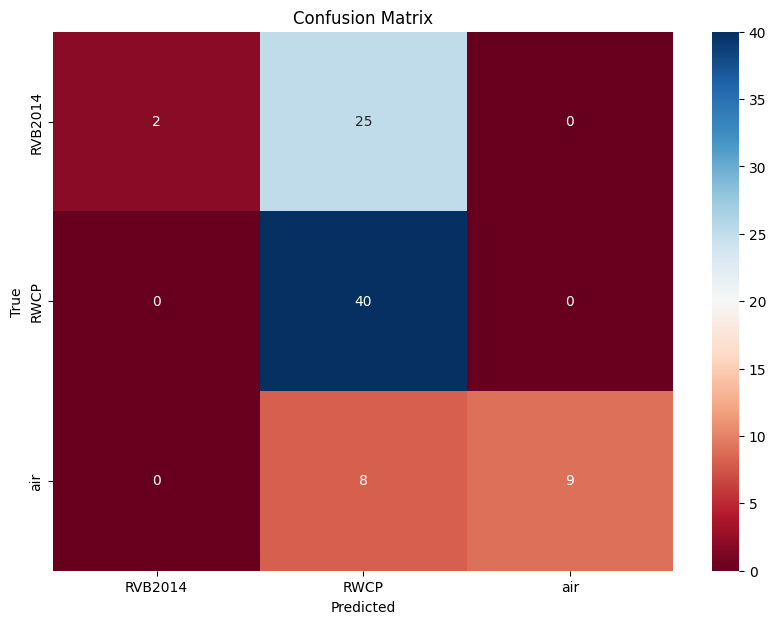
\includegraphics[width=\textwidth]{confusion_matrix.png}
\caption{Confusion matrix heatmap showing true vs. predicted classifications.}
\label{fig:confusion_matrix}
\end{figure}

\begin{figure}[H] % Use H to force placement
\centering
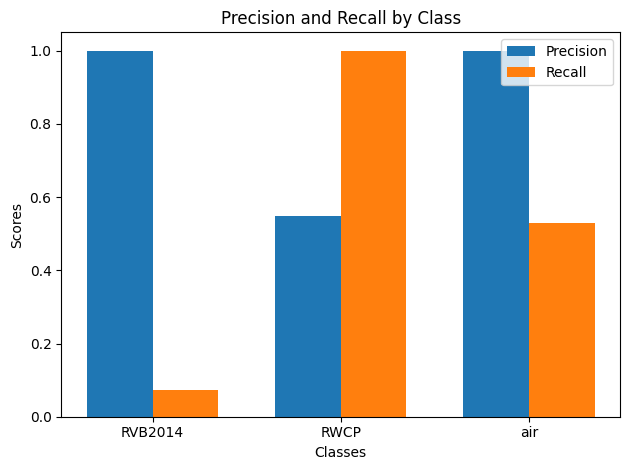
\includegraphics[width=\textwidth]{precision_recall.png}
\caption{Precision and recall bar chart by class.}
\label{fig:precision_recall}
\end{figure}

\begin{figure}[H] % Use H to force placement
\centering
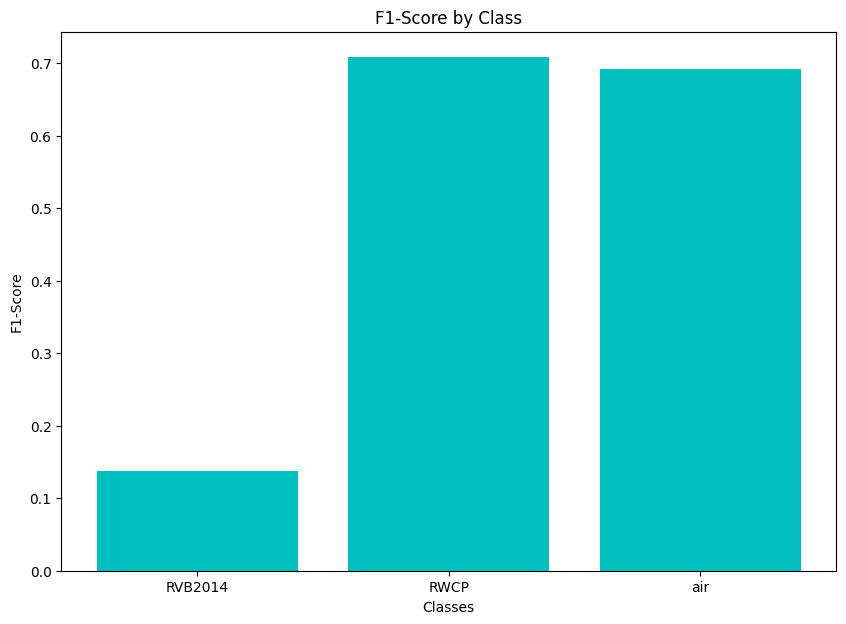
\includegraphics[width=\textwidth]{f1_score.png}
\caption{F1-score bar chart by class.}
\label{fig:f1_score}
\end{figure}

\section{Conclusion}
For the most part, the project was a process. I started with the idea of a simple CNN-SVM hybrid audio classification system. Over time, the project evolved. First, I was able to learn some new techniques for audio processing from a couple of papers, then I had to go through the process of making my models work cohesively together. This was the longest process. Finally, I had to find a way to train the model - given the computing resources I had. Initially, I was hoping to gain access to the San Diego Supercomputer (SDSC). However, this proved to not be an option. Thus, I learned several ways to optimize the resources that I had to perform computations. Thus, we arrive at the end product. I believe my project demonstrates the potential effectiveness of combining CNNs with SVMs for audio classification of disentangled signals. Overall, I was pleasantly surprised by the overall accuracy result of 85\%. Future work could be done in exploring additional feature extraction methods and more complex hybrid models. Maybe this could eventually lead to instrument recognition?

\section{Supplementary Materials}
\subsection{Code}
The complete code for this project is available at \url{https://github.com/NehemiahSkan/CSE_192_Project}.

\bibliography{references}


\end{document}